\documentclass{article}
%% This is the preamble
    \usepackage[utf8]{inputenc}
    \usepackage[dvipsnames,svgnames,x11names,table]{xcolor}
    %% To customize page margins, use geometry
    \usepackage{geometry}
    \geometry{top=1.5in,left=1in, right=1in, bottom = 1.5in}
    %% physics and math packages
    \usepackage{amsmath,derivative,siunitx}
    %% some helpful packages to make internal links in your document
    \usepackage{hyperref}
    %% to include pictures and plots
    \usepackage{graphicx}
    % extra packages for Quantum
    \usepackage{braket}
    \renewcommand{\doteq}{\,\dot{=}\,}


\title{Homework 5}
\author{Adrian deCola}
\date{April 5, 2023}


%% Now we begin the formal document
\begin{document}

\maketitle


\section*{Problem 10.44}
\verb+Problem+: An axially symmetric space station (principal axis $\boldsymbol{e}_3$, and $\lambda_1 = \lambda_2$) is floating in free space. It has rockets mounted symmetrically on either side that are firing and exert a constant torque $\Gamma$ about the symmetry axis. Solve Euler's equations exactly for $\boldsymbol{\omega}$ (relative to the body axis) and describe the motion. At $t = 0$ take $\boldsymbol{\omega} = (\omega_{10} , 0, \omega_{30})$.


\begin{figure}[!h]
    \centering
    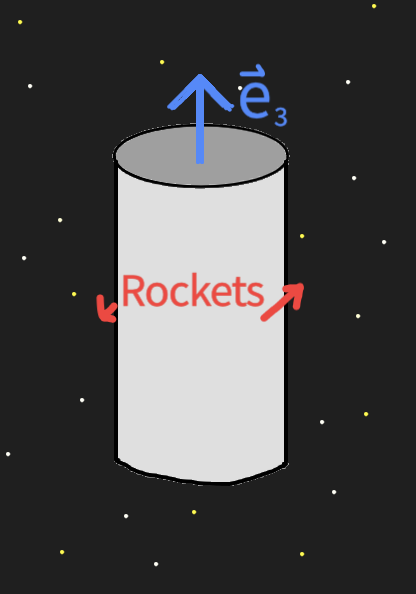
\includegraphics[width=.45\textwidth]{hw5_fig1.png}
    \caption{An illustration of what the space station could look like.}
\end{figure}


\hrule
         \ \ \ 
\\
\\
As the question states, we will use Euler's equations as shown below to describe the motion. 
\begin{figure}[!h]
    \centering
    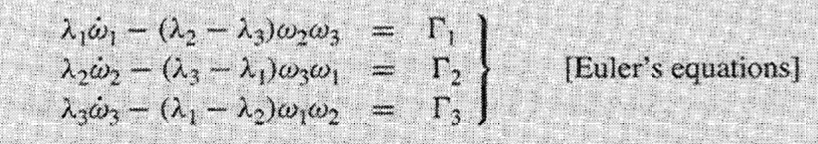
\includegraphics[width=.8\textwidth]{hw5_fig2.png}
\end{figure}
\\
The torque is only around the symmetric axis. 
$$\boldsymbol{\Gamma}=(0, 0, \Gamma )$$
Therefore, $\Gamma_1=0$, $\Gamma_1=0$, and $\Gamma_3=\Gamma$. Since the space station is axially symmetric around the principle axis, $\lambda_1 = \lambda_2$. Substituting these results into our Euler equations we find: 

\begin{align*}
    \lambda_1 \dot{\omega}_1 &= (\lambda_1-\lambda_3)\omega_2 \omega_3 \\
    \lambda_1 \dot{\omega}_2 &= (\lambda_3-\lambda_1)\omega_1 \omega_3 \\
    \lambda_3 \dot{\omega}_3 &= \Gamma
\end{align*}
Solving the third equation for $\omega_3$ we find: 
\begin{align*}
    \lambda_3 \dot{\omega}_3 &= \Gamma \\
    \dot{\omega}_3 &= \frac{\Gamma }{\lambda_3} \\
    \int_{\omega_{30}}^{\omega_3}\dot{\omega}_3 dt &= \int_0^t{\frac{\Gamma }{\lambda_3}}dt \\
    \omega_3 &= \frac{\Gamma }{\lambda_3}t + \omega_{30}
\end{align*}
$$\boxed{\omega_3(t) = \frac{\Gamma }{\lambda_3}t + \omega_{30}}$$
This describes the rotation about the principle axis, which we will interpret later with the other angular velocities about the principle axes. Substituting this into our other Euler equations we find:

\begin{align*}
    \dot{\omega}_1 &= \frac{\lambda_1-\lambda_3}{\lambda_1}\left( \frac{\Gamma }{\lambda_3}t + \omega_{30} \right) \omega_2 \\
    \dot{\omega}_2 &= -\frac{\lambda_1-\lambda_3}{\lambda_1}\left( \frac{\Gamma }{\lambda_3}t + \omega_{30} \right) \omega_1 \\
\end{align*}
To solve these coupled equations for $\omega_1$ and $\omega_2$, we will define the complex number $\eta$.
$$\eta = \omega_1 + i\omega_2$$
It is clear that $\omega_1 = Re(\eta)$ and $\omega_2 = Im(\eta)$. As we have $\dot{\omega}_1$ and $\dot{\omega}_2$ separated, we will solve for $\dot{\eta} = \dot{\omega}_1 + i\dot{\omega}_2$. 

\begin{align*}
    \dot{\eta} &= \frac{\lambda_1-\lambda_3}{\lambda_1}\left( \frac{\Gamma }{\lambda_3}t + \omega_{30} \right) \omega_2 + i \left( -\frac{\lambda_1-\lambda_3}{\lambda_1}\left( \frac{\Gamma }{\lambda_3}t + \omega_{30} \right) \omega_1\right)  \\
    \dot{\eta} &= \frac{\lambda_1-\lambda_3}{\lambda_1}\left( \frac{\Gamma }{\lambda_3}t + \omega_{30} \right) (\omega_2-i\omega_1) \\
    \dot{\eta} &= \frac{\lambda_1-\lambda_3}{\lambda_1}\left( \frac{\Gamma }{\lambda_3}t + \omega_{30} \right) (-i)(\omega_1+i\omega_2) \\
    \dot{\eta} &= \frac{\lambda_1-\lambda_3}{\lambda_1}\left( \frac{\Gamma }{\lambda_3}t + \omega_{30} \right) (-i\eta) \\
    \dot{\eta} &= i\left[ \frac{\lambda_3-\lambda_1}{\lambda_1}\left( \frac{\Gamma }{\lambda_3}\right) t  +  \frac{\lambda_3-\lambda_1}{\lambda_1}\omega_{30} \right] \eta \\
\end{align*}
Seeing a differential equation of this form, it looks like our solution should be in the form of an exponential. Specifically, we should use one of the following form to also get a polynomial product when we differentiate:

\begin{align*}
    \eta &= Ae^{i(\alpha t^2 + \beta t)} \\
\end{align*}
Differentiating we find:

\begin{align*}
    \dot{\eta} &=A (2\alpha t + \beta ) e^{i(\alpha t^2 + \beta t)} \\
    \dot{\eta} &=i(2\alpha t + \beta ) (Ae^{i(\alpha t^2 + \beta t})) \\
    \dot{\eta} &=i(2\alpha t + \beta ) \eta \\
\end{align*}
This is in the same form as our differential equations above where $2\alpha = \frac{\lambda_3-\lambda_1}{\lambda_1}\left( \frac{\Gamma }{\lambda_3}\right)$ and $\beta = \frac{\lambda_3-\lambda_1}{\lambda_1}\omega_{30}$. Isolating $\alpha$:

\begin{align*}
    \alpha &= \frac{\lambda_3-\lambda_1}{\lambda_1}\left( \frac{\Gamma }{2\lambda_3}\right) 
\end{align*}
To find $A$, we will use our initial condition(s) that $\omega_1(0) = \omega_{10}$ and  $\omega_2(0) = 0$. 


\begin{align*}
    \eta(0) &= \omega_1(0) + i\omega_2(0) \\
    Ae^{i(\alpha (0)^2 + \beta (0))} &= \omega_{10} \\
    A &= \omega_{10} \\
\end{align*}
Substituting in the values we found for $A$, $\alpha$, and $\beta$; we now know $\eta$. 

\begin{align*}
    &\eta = \omega_{10}  exp\left[ i\left( \frac{\lambda_3-\lambda_1}{\lambda_1}\left( \frac{\Gamma }{2\lambda_3}\right)t^2 + \frac{\lambda_3-\lambda_1}{\lambda_1}\omega_{30} t\right) \right] \\
    &\eta = \omega_{10} cos\left( \frac{\lambda_3-\lambda_1}{\lambda_1}\left( \frac{\Gamma }{2\lambda_3}\right)t^2 + \frac{\lambda_3-\lambda_1}{\lambda_1}\omega_{30} t \right) + i \omega_{10} sin\left( \frac{\lambda_3-\lambda_1}{\lambda_1}\left( \frac{\Gamma }{2\lambda_3}\right)t^2 + \frac{\lambda_3-\lambda_1}{\lambda_1}\omega_{30} t \right)
\end{align*}
We can also use this to solve for $\omega_1$ and $\omega_2$.

\begin{align*}
    &\omega_1 = Re(\eta) \\
    &\boxed{\omega_1(t) = \omega_{10} cos\left( \frac{\lambda_3-\lambda_1}{\lambda_1}\left( \frac{\Gamma }{2\lambda_3}\right)t^2 + \frac{\lambda_3-\lambda_1}{\lambda_1}\omega_{30} t \right)} \\
    &\omega_2 = Im(\eta) \\
    &\boxed{\omega_2(t) =\omega_{10} sin\left( \frac{\lambda_3-\lambda_1}{\lambda_1}\left( \frac{\Gamma }{2\lambda_3}\right)t^2 + \frac{\lambda_3-\lambda_1}{\lambda_1}\omega_{30} t \right)} \\
\end{align*}
We will also reiterate the result for $\omega_3$ for reference. 
$$\boxed{\omega_3(t) = \frac{\Gamma }{\lambda_3}t + \omega_{30}}$$
Plugging these results into the original Euler equations we see that they are solutions. We also see that all the dimensions are consistent. Rotation about the third principle axis will grow linearly over time. This makes sense as we apply a constant torque along this axis and it is, of course, a principle axis. Rotation about the first principle axis, starts with its initial rotation and then oscillates back and forth between rotating with this initial rotational velocity in the opposite direction sinusoidally with this oscillation happening faster and faster over time. The rocket starts off not rotating about the second principle axis but then oscillated between a rotational velocity, with a maximum amplitude of the initial rotational velocity about the first principle axis, sinusoidally and also oscillating faster over time. In other words, the initial rotational velocity about the first principle axis oscillates between the first and second principle axis, sinusoidally, oscillating faster and faster over time. This is an important thing to consider. A slight rotational velocity about the wrong axis, could cause jostling over time if we fire other rockets to cause rotational acceleration. 




\subsection*{Citation}
(1) Taylor, John R. Classical Mechanics. University Science Books, 2014. 

\end{document}